\chapter{VR and Education}
\label{chap:vreducation}

With the onset of new HMD technology driven by the Oculus Rift, VR is now expanding rapidly at the hands of brilliant engineers and researchers. This technology has grown so much in the past few years that research is finally beginning to surface regarding applications of VR beyond the stereotypical realm of gaming. Advancements in VR technology have allowed for a myriad of disciplines to integrate the technology into their own practices to create stunning results. In particular, the realm of education has been latching onto the concept of VR as a means for redefining how skills can be taught in the modern world. 

\section{Surgery}
\label{sec:surgery}

From an educational standpoint VR offers a wide variety of opportunities for learning. In particular, one of the largest applicational fields for VR as an educational tool is surgery. In the realm of health sciences, surgery is a very technical outlet that requires precise motor movements in order to be performed successfully. Obviously due to the high risk of failure associated with surgery (the risk of the patients' lives), the practice of surgical training is taken both seriously, and enthusiastically. Research on the topic of improving surgical training and skill is bountiful, and frequently carried out through high budget projects from the National Institute of Health (NIH).

As mentioned in Section 2.1, the 1990s was a decade in which VR technology was first brought to mass media attention. It was noted that most of these technologies were unrealistic and public attention to the topic began to fade. In the wake of this media fallout VR development and research returned primarily to its historical roots of DoD and NASA funding, with a few exceptions. The largest of these exceptions was the NIH, which began seriously investigating the use of VR as a tool for training surgeons \cite{soriano_systematic_2011}. 

More specifically, the NIH was interested in the effects of VR in conjunction with laparoscopic surgery. As a brief overview, laparoscopic surgery is also commonly referred to as minimally invasive surgery (MIS), and it involves a very technical approach to surgery. Rather than approaching a surgical site directly and possibly involving messy insertions, MIS surgeries take place far from their operation location through small incision points (centimeters in length) elsewhere in the body. From these insertion sites a lengthy fiber optic cable system known as a laparoscope is inserted and directed to the operation site. This approach to surgery is highly preferred when it can be performed, as pain and hemorrhaging are greatly reduced due to the smaller incisions, and moreover recovery time is reduced as well. The actual surgery often takes place with the aid of a video camera attached to the laparoscope, whose output is fed to a monitor for the surgeon to use as their primary sight for the operation.

One can see why the NIH would be interested in improving laparoscopic surgery, and why they would be concerned with providing the best educational training available for laparoscopic surgeons. In this particular case, the NIH performed a lengthly series of research studies on using VR specifically to train laparoscopic surgeons, and moreover to determine if training through VR was effective \cite{westwood_medicine_1998}.

The NIH first began this research in 1998 when they developed a system called MIST VR. MIST VR was a unique VR simulation made to model the movements needed to perform MIS, and it could also judge and score a user's particular skill in performing the surgery. The scoring system embedded in MIST VR was groundbreaking for numerous reasons, but mostly because before this there was no way to quantify a particular laparoscopic surgeons "skill". With MIST VR, the NIH found that the most experienced laparoscopic surgeons scored the highest, and correspondingly surgeons with less experience scored lower on a geometric progression. More interestingly, though, the NIH found that surgeons who trained with MIST VR became more efficient and saw a reduction in errors while performing roughly at the same speed. Thus, the NIH found that through VR they were able to assess a particular surgeon's skill level, and also found a significant beneficial effect of training within VR compared to traditional methods \cite{gallagher_virtual_2005}.

Ever since the preliminary work done with VR as a tool for health training by the NIH in 1998, the NIH has continued similar research. However, with the advent of recent VR advancements, a myriad of new research projects using VR for health applications are starting to emerge. For example, a surgical training program in France has begun research into using VR to help assist in surgical training for open surgeries, rather than solely laparoscopic surgeries. This group is attempting to address a common problem in surgical training, which revolves around young surgeons not getting the most out of observational surgeries. Essentially, when a surgeon is in their early training they often stand in the operation room with an experienced surgeon and observe the experienced surgeon perform a full surgery. The surgeon in training, however, must remain out of the way for obvious safety concerns, and are forced to look over a crowded scene and try to make sense of what they are seeing.

There is room for advancement in this area, and a group in France is attempting to solve this common problem through VR. What they have done is quite fascinating: by taking two head mounted cameras and positioning them such that they mimic human eye placements, they can record an entire surgery and then later alter the video feeds such that they can be observed through a VR HMD. A user can then watch the entire video feed as if they are seeing the recorded footage through their own eyes, and can even hear after edited audio layered onto the scene. This means that these surgeons in training can now observe an entire surgery from the view point of the lead surgeon like never before, and more importantly they can listen to the lead surgeon as he explains his every move. Figure~\ref{figure:f_surgery} demonstrates the camera rig used by the lead surgeon in action.

\begin{figure}
  \centering
  %\begin{picture}
  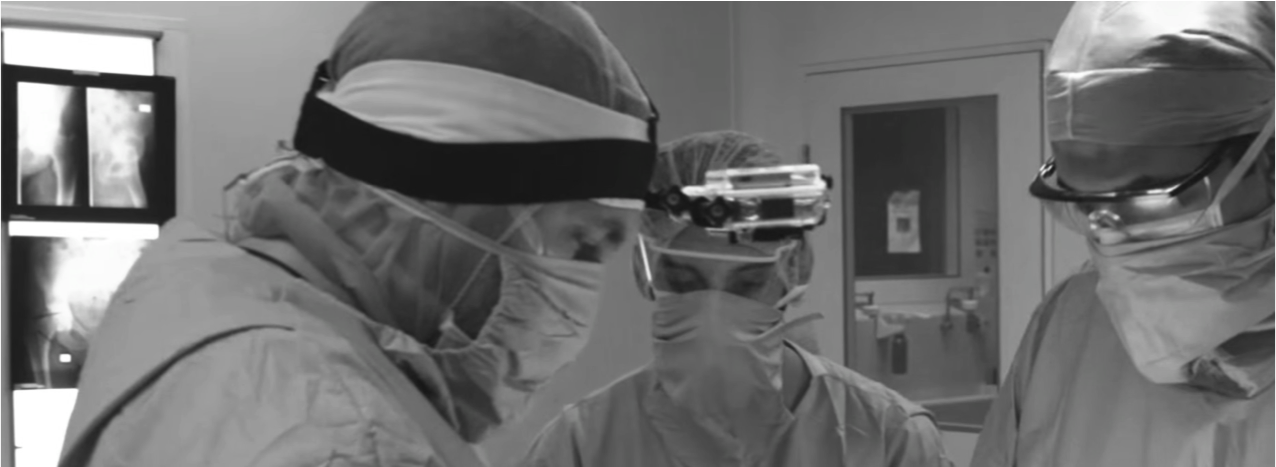
\includegraphics[scale=.50]{img_surgery}
  %\end{picture}
  \caption{Lead surgeon wearing VR camera rig.}
  \label{figure:f_surgery}
\end{figure}
%Figure~\ref{figure:f_dk1}

Clearly these studies show that VR can be used in a professional setting such as surgical training. More importantly, these studies show that VR can be used to teach incredibly necessary skills for these professions, and in certain circumstances VR is a better way to learn these skills rather than otherwise. Finally, in further research done by the NIH it was concluded that VR when used for proficiency-based training is presenting itself as a paradigm shift in surgical skills training \cite{seymour_virtual_2002}.

\section{Military Training}
\label{sec:military}

As was mentioned in chapter 2, one of the largest funders and adopters of VR technology for educational purposes has always been the United States' Department of Defense. The technology makes obvious sense for military training purposes, as it allows personnel to train for potentially hostile environments that are difficult to recreate in person. By using VR, the military can carry out combat training with absolutely no risk of failure, and can even use VR to help expose these soldiers to potentially life threatening situations in a completely controlled environment. 

The military has been using VR since its early days in the 1960s, and has found the technology paramount for training simulations. Besides solely combat training, the military has used VR enthusiastically for training pilots. This is a natural usage extension from combat training, as VR can be used to create realistic flight simulations in which pilots in training can be exposed to a lifelike simulation with no risk of failure. In this case, VR is exceptionally useful, as failure in a real test case could potentially mean both loss of life and loss of expensive aircraft. Currently, VR pilot simulations are used in conjunction with extensive Augmented Reality (AR) controllers meant to closely mimic the actual instrumentation used by pilots. Because of this, the VR simulation is an even more effective training simulation, as the pilot in training is immersed not just visually but also in a tactile manner,  increasing the sense of presence, and thus the effectiveness. 

\section{Stem}
\label{sec:stem}

With the recent advancements in VR technology, the landscape of VR research and applications is quickly changing. For the first time, affordable and powerful HMDs are available to the public and the resulting applications that have been built using the technology have been increasingly impressive. While a great many of these applications are simply video games, quite a few are educational in nature. 

A great example of a popular free application for the Oculus Rift is the extraordinary free application \textit{Titans of Space}. In this application the player assumes the role of an astronaut in a spaceship which tours our solar system and gives an educational guide to the surrounding planets and stars. The simulation excels by providing a realistic scale to the astral bodies, which helps the player realize through their own sight just how big these astral bodies are, especially compared to each other. As seen in Figure~\ref{figure:f_space}, while the player is touring our solar system, the only prominent part of their spaceship in view is a display which lists educational facts and a brief synopsis of each solar body. 

\begin{figure}
  \centering
  %\begin{picture}
  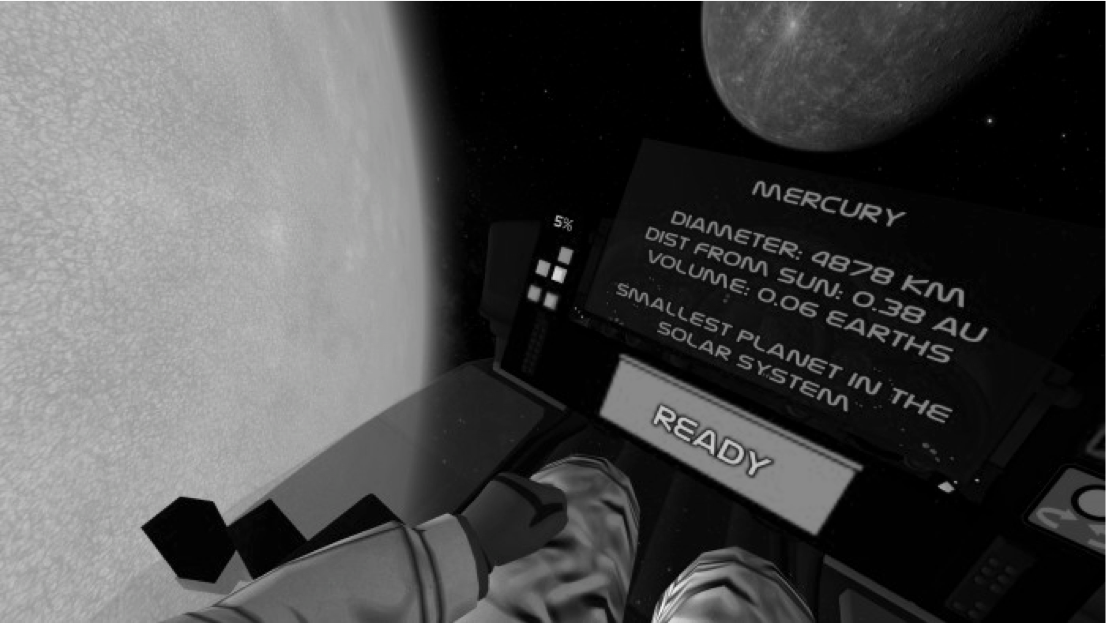
\includegraphics[scale=.75]{img_titans}
  %\end{picture}
  \caption{Screenshot of Titans of Space.}
  \label{figure:f_space}
\end{figure}
%Figure~\ref{figure:f_dk1}

Clearly this application is an example of a STEM based VR application, and games like these can be used to inspire creative thinking \cite{merchant_effectiveness_2014}. Applications such as this one could be used to re-interest students in STEM fields through new integration with exciting technology which increases student motivation to learn. As time progresses and HMD technology continues to develop, the number of educational simulations such as this will continue to grow, and if used appropriately in the classroom could be an exciting way to approach a topic.